% Options for packages loaded elsewhere
% Options for packages loaded elsewhere
\PassOptionsToPackage{unicode}{hyperref}
\PassOptionsToPackage{hyphens}{url}
%
\documentclass[
  ignorenonframetext,
]{beamer}
\newif\ifbibliography
\usepackage{pgfpages}
\setbeamertemplate{caption}[numbered]
\setbeamertemplate{caption label separator}{: }
\setbeamercolor{caption name}{fg=normal text.fg}
\beamertemplatenavigationsymbolsempty
% remove section numbering
\setbeamertemplate{part page}{
  \centering
  \begin{beamercolorbox}[sep=16pt,center]{part title}
    \usebeamerfont{part title}\insertpart\par
  \end{beamercolorbox}
}
\setbeamertemplate{section page}{
  \centering
  \begin{beamercolorbox}[sep=12pt,center]{section title}
    \usebeamerfont{section title}\insertsection\par
  \end{beamercolorbox}
}
\setbeamertemplate{subsection page}{
  \centering
  \begin{beamercolorbox}[sep=8pt,center]{subsection title}
    \usebeamerfont{subsection title}\insertsubsection\par
  \end{beamercolorbox}
}
% Prevent slide breaks in the middle of a paragraph
\widowpenalties 1 10000
\raggedbottom
\AtBeginPart{
  \frame{\partpage}
}
\AtBeginSection{
  \ifbibliography
  \else
    \frame{\sectionpage}
  \fi
}
\AtBeginSubsection{
  \frame{\subsectionpage}
}
\usepackage{iftex}
\ifPDFTeX
  \usepackage[T1]{fontenc}
  \usepackage[utf8]{inputenc}
  \usepackage{textcomp} % provide euro and other symbols
\else % if luatex or xetex
  \usepackage{unicode-math} % this also loads fontspec
  \defaultfontfeatures{Scale=MatchLowercase}
  \defaultfontfeatures[\rmfamily]{Ligatures=TeX,Scale=1}
\fi
\usepackage{lmodern}

\usetheme[]{metropolis}
\ifPDFTeX\else
  % xetex/luatex font selection
\fi
% Use upquote if available, for straight quotes in verbatim environments
\IfFileExists{upquote.sty}{\usepackage{upquote}}{}
\IfFileExists{microtype.sty}{% use microtype if available
  \usepackage[]{microtype}
  \UseMicrotypeSet[protrusion]{basicmath} % disable protrusion for tt fonts
}{}
\makeatletter
\@ifundefined{KOMAClassName}{% if non-KOMA class
  \IfFileExists{parskip.sty}{%
    \usepackage{parskip}
  }{% else
    \setlength{\parindent}{0pt}
    \setlength{\parskip}{6pt plus 2pt minus 1pt}}
}{% if KOMA class
  \KOMAoptions{parskip=half}}
\makeatother


\usepackage{longtable,booktabs,array}
\usepackage{calc} % for calculating minipage widths
\usepackage{caption}
% Make caption package work with longtable
\makeatletter
\def\fnum@table{\tablename~\thetable}
\makeatother
\usepackage{graphicx}
\makeatletter
\newsavebox\pandoc@box
\newcommand*\pandocbounded[1]{% scales image to fit in text height/width
  \sbox\pandoc@box{#1}%
  \Gscale@div\@tempa{\textheight}{\dimexpr\ht\pandoc@box+\dp\pandoc@box\relax}%
  \Gscale@div\@tempb{\linewidth}{\wd\pandoc@box}%
  \ifdim\@tempb\p@<\@tempa\p@\let\@tempa\@tempb\fi% select the smaller of both
  \ifdim\@tempa\p@<\p@\scalebox{\@tempa}{\usebox\pandoc@box}%
  \else\usebox{\pandoc@box}%
  \fi%
}
% Set default figure placement to htbp
\def\fps@figure{htbp}
\makeatother





\setlength{\emergencystretch}{3em} % prevent overfull lines

\providecommand{\tightlist}{%
  \setlength{\itemsep}{0pt}\setlength{\parskip}{0pt}}



 


\setbeamerfont{title}{size=\large}
\makeatletter
\@ifpackageloaded{caption}{}{\usepackage{caption}}
\AtBeginDocument{%
\ifdefined\contentsname
  \renewcommand*\contentsname{Table of contents}
\else
  \newcommand\contentsname{Table of contents}
\fi
\ifdefined\listfigurename
  \renewcommand*\listfigurename{List of Figures}
\else
  \newcommand\listfigurename{List of Figures}
\fi
\ifdefined\listtablename
  \renewcommand*\listtablename{List of Tables}
\else
  \newcommand\listtablename{List of Tables}
\fi
\ifdefined\figurename
  \renewcommand*\figurename{Figure}
\else
  \newcommand\figurename{Figure}
\fi
\ifdefined\tablename
  \renewcommand*\tablename{Table}
\else
  \newcommand\tablename{Table}
\fi
}
\@ifpackageloaded{float}{}{\usepackage{float}}
\floatstyle{ruled}
\@ifundefined{c@chapter}{\newfloat{codelisting}{h}{lop}}{\newfloat{codelisting}{h}{lop}[chapter]}
\floatname{codelisting}{Listing}
\newcommand*\listoflistings{\listof{codelisting}{List of Listings}}
\makeatother
\makeatletter
\makeatother
\makeatletter
\@ifpackageloaded{caption}{}{\usepackage{caption}}
\@ifpackageloaded{subcaption}{}{\usepackage{subcaption}}
\makeatother

\usepackage{bookmark}
\IfFileExists{xurl.sty}{\usepackage{xurl}}{} % add URL line breaks if available
\urlstyle{same}
\hypersetup{
  pdfauthor={Giorgio Arcara},
  hidelinks,
  pdfcreator={LaTeX via pandoc}}


\author{Giorgio Arcara}
\date{}

\begin{document}


\begin{frame}
% TITLE SLIDES
\title{Metodi Statistici per la Neuropsicologia Forense\\ \vspace{1em} \small \emph{4a. Validità e affidabilità (teoria)}}
\author{Giorgio Arcara,\\ Università di Padova \\ IRCCS San Camillo, Venezia}

\titlegraphic{

\vspace*{7cm}

\includegraphics[scale=0.15]{Figures/LogoSanCamilloIRCCS_Unipd_alpha.png}
\hfill 
\includegraphics[scale=0.15]{Figures/CC_license_3_0.png}
}
\maketitle
\end{frame}

\section{Validità e affidabilità}\label{validituxe0-e-affidabilituxe0}

\begin{frame}{Validità e Affidabilità}
\phantomsection\label{validituxe0-e-affidabilituxe0-1}
\small
\begin{columns}
\column{0.8\textwidth}
Validità e affidabilità sono due qualità fondamentali dei test (non solo didatticamente).
\column{0.2\textwidth}
\begin{figure}
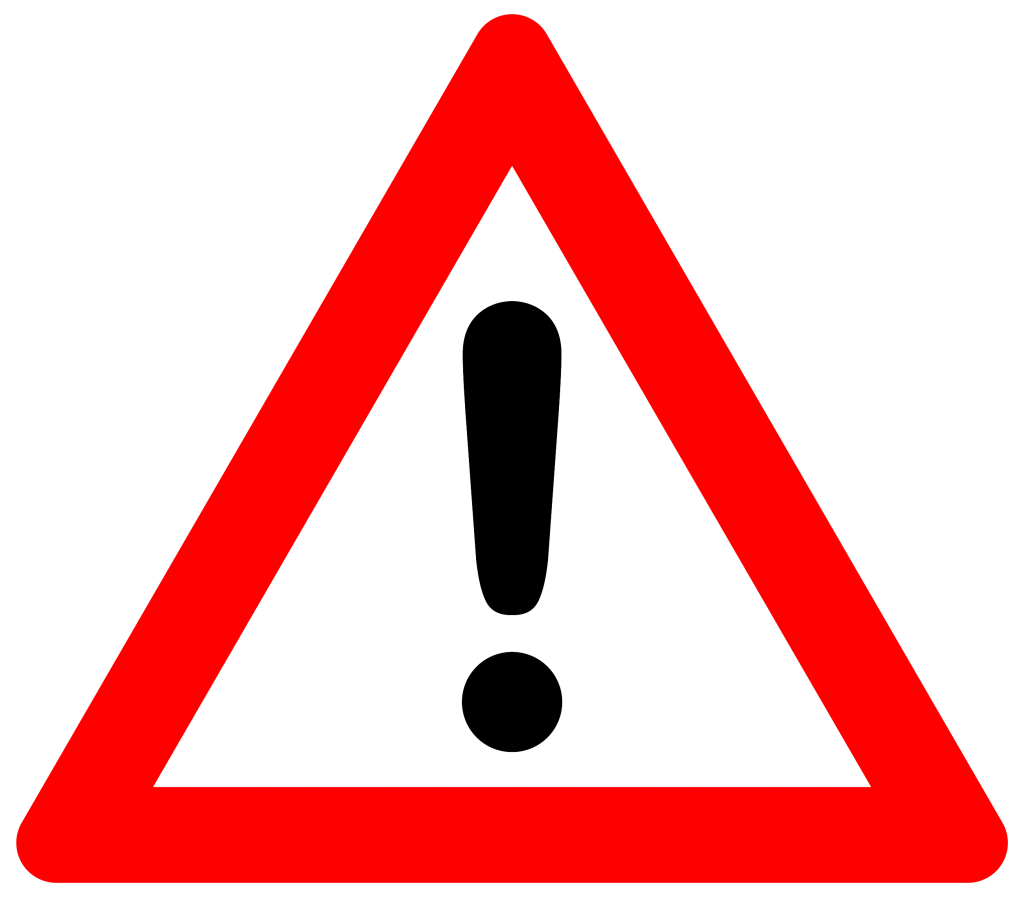
\includegraphics[scale=0.05]{Figures/triangle.png}
\end{figure}
\end{columns}

\vfill

Nelle prossime slides farà una panoramica generale senza scendere nei
dettagli delle formule che vedremo in un passo successivo.
\end{frame}

\begin{frame}{Validità e affidabilità}
\phantomsection\label{validituxe0-e-affidabilituxe0-2}
Usare un test senza conoscerne validità e affidabilità può portare a
grossi errori:

Per dare un'analogia (estrema) usare un test con bassa affidabilità e
nessuna validità per un interpretazione per un'interpretazione e
potrebbe portare a misurare l'altezza di una persona con una bilancia
che ha un margine di errore di 10 kg.

\textbf{Dal momento che i test sono strumenti di misurazione non
possiamo prescindere dal conoscerne le loro qualità.}
\end{frame}

\begin{frame}{Validità e affidabilità (brevi definizioni)}
\phantomsection\label{validituxe0-e-affidabilituxe0-brevi-definizioni}
La \textbf{validità} è la qualità di un test di misurare effettivamente
il costrutto che vuole misurare.

L' \textbf{affidabilità} indica la precisione di un test.
\end{frame}

\begin{frame}{Come vorremmo fossero Validità e Affidabilità (ma non
sono)}
\phantomsection\label{come-vorremmo-fossero-validituxe0-e-affidabilituxe0-ma-non-sono}
\textbf{Validità}: il mio test misura il mio costrutto in maniera nota e
quantificabile. Es.:

\begin{itemize}
\tightlist
\item
  l'80\% del punteggio osservato è riconducibile al construtto di
  interesse
\item
  il punteggio riconducibile al costrutto di interesse mentre +/-5\% ad
  altri costrutti.
\end{itemize}

\vfill
\pause

\textbf{Affidabilità}: il mio test misura il mio costrutto con
precisione quantificabile. Es.:

\begin{itemize}
\tightlist
\item
  il mio punteggio finale può essere sbagliato di +/-3
\item
  il punteggio finale puà essere sbagliato di +/-5\%
\end{itemize}
\end{frame}

\begin{frame}{Come vorremmo fossero Validità e Affidabilità (ma non
sono)}
\phantomsection\label{come-vorremmo-fossero-validituxe0-e-affidabilituxe0-ma-non-sono-1}
Anche se ci sono dei criteri talvolta di soglia minima (di affidabilità
o validità) non c'è una unanimità. éer considerare un test adeguato,
spesso questi valori ci aiutano a distinguere test tra di loro, per
scegliere il migliore (o il meno peggiore)

\vfill

\begin{center}
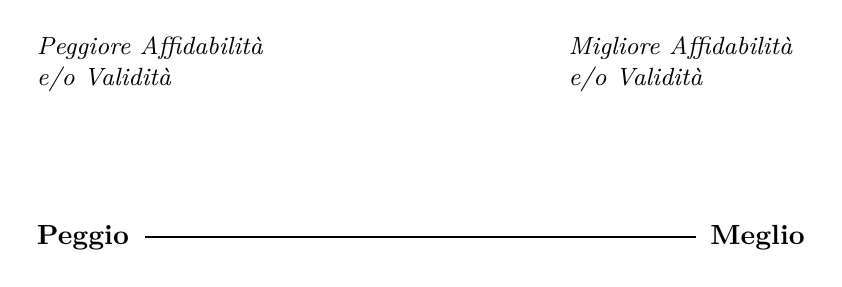
\begin{tikzpicture}[baseline=(current bounding box.center)]


% : peggio - meglio
\node[anchor=west] at (0, 1) {\small \parbox{3cm}{\emph{Peggiore Affidabilità \\e/o Validità}}};
\node[anchor=east] at (10, 1) {\small \parbox{3cm}{\emph{Migliore Affidabilità \\e/o Validità}}};


\node[anchor=west] at (0, -1.2) {\textbf{Peggio}};
\node[anchor=east] at (10, -1.2) {\textbf{Meglio}};
\draw[thick] (1.5, -1.2) -- (8.5, -1.2);

\end{tikzpicture}
\end{center}
\end{frame}

\section{Validità}\label{validituxe0}

\begin{frame}{Parlare correttamente di validità}
\phantomsection\label{parlare-correttamente-di-validituxe0}
La validità è la qualità di un test di misurare ciò che effettivamente
vuole misurare. Il termine validità è sempre riferito ad
un'\textbf{utilizzo} che si fa dei punteggi. \vfill \pause Non ha senso
dire che \textbf{un test è valido} \vfill \pause

\begin{center}
\tikz[baseline=(t.base)]{
  \node[inner sep=0pt, outer sep=0pt, anchor=base] (t)
    {\emph{"usa questo test! è stato validato!"}};
  \draw[red, thick] ([yshift=0.4em]t.south west) -- ([yshift=0.4em]t.south east);
}
\end{center}
\end{frame}

\begin{frame}{Un concetto da ribadire}
\phantomsection\label{un-concetto-da-ribadire}
\begin{center}
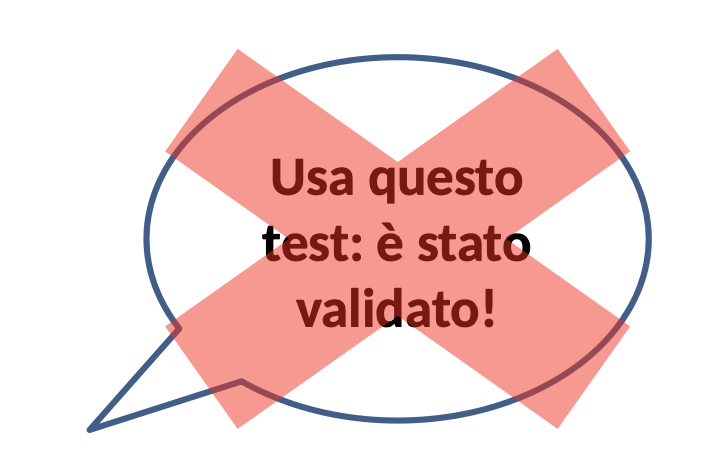
\includegraphics[width=0.5\linewidth,height=\textheight,keepaspectratio]{Figures/Usa_questo_test.png}
\end{center}
\end{frame}

\begin{frame}{La Validità}
\phantomsection\label{la-validituxe0}
Un test può avere validità per una certa utilizzo o per più utilizzi.

La validità non è una qualità tutto-o-nulla, ma una qualità lungo un
continuum

Ad esempio ci sono evidenze che il \emph{''Free and Cued Selective
Reminding Test-it''} (Clerici et al., 2017) è un test con buona validità
per misurare le capacità di memoria.
\end{frame}

\begin{frame}{La Validità (non dimostrata)}
\phantomsection\label{la-validituxe0-non-dimostrata}
talvolta, alcuni test non riportano nessun evidenza di validità. Si
tratta di strumenti in cui non abbiamo la certezza di cosa stiano
misurando.
\end{frame}

\begin{frame}{Tipi di validità}
\phantomsection\label{tipi-di-validituxe0}
\begin{itemize}
\tightlist
\item
  Validità di facciata
\item
  Validità di contenuto
\item
  Validità convergente/divergente (validità di costrutto)
\item
  Validità di criterio
\item
  Validità concorrente
\item
  Validità ecologica
\end{itemize}

Esistono diverse classificazioni di validità e affidabilità (vedi
Urbina, 2004, Essentials of Psychological Testing, per un
approfondimento). Quelle che segue è solo una delle possibili
classificazioni.
\end{frame}

\begin{frame}{Validità a priori e a posteriori}
\phantomsection\label{validituxe0-a-priori-e-a-posteriori}
La validità è distinta anche in \emph{a priori} e \emph{a posteriori} La
validità a priori è quella che si può esaminare prima che si abbiano
dati empirici sul test. (lo sono, la validità di facciata e la validità
di contenuto). La validità a posteriori è invece quella che si può
valutare solo quando sono disponibili dati sul test (lo sono la validità
di costrutto, la validità di criterio e la validità ecologica.)
\end{frame}

\begin{frame}{Validità di facciata 1/2}
\phantomsection\label{validituxe0-di-facciata-12}
Validità di facciata: si riferisce alla qualità di un test di esssere
chiaramente riconducibile al costrutto che vuole misurare. Es. un test
di memoria che richiede di ricordare gli items.

Talvolta è l'unico tipo di validità che abbiamo a disposizione (ma di
cui non dovremmo accontentarci.)

Data la natura prettamente qualitativa non esistono analisi per
verificarla.
\end{frame}

\begin{frame}{Validità di facciata 2/2}
\phantomsection\label{validituxe0-di-facciata-22}
La plausibilità di una misurazione non è sufficiente per giudicare se
effettivamente stiamo misurando quello che ci interessa.

\pandocbounded{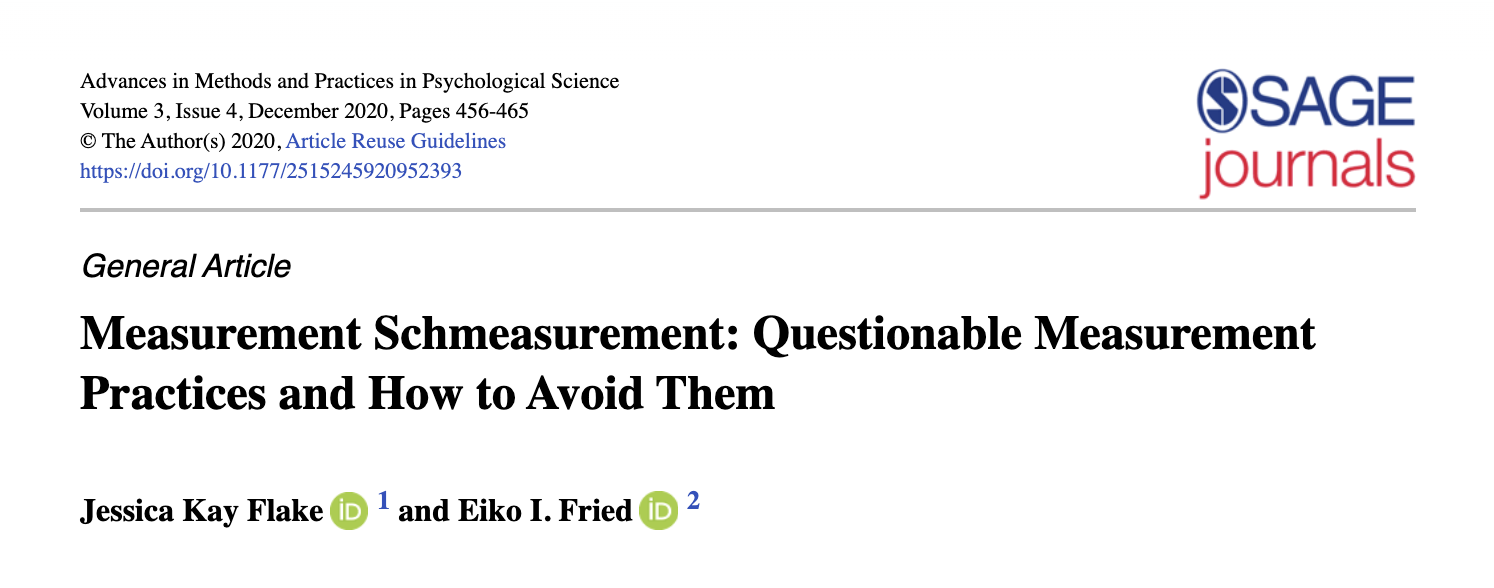
\includegraphics[keepaspectratio]{Figures/QMP.png}}
\end{frame}

\begin{frame}{Validità di contenuto 1/2}
\phantomsection\label{validituxe0-di-contenuto-12}
Validità di contenuto : la proprietà degli item di essere sufficienti ed
adeguati per valutare il costrutto di interesse. Può essere valutata
qualitativamente o quantitativamente (Lawshe, 1975).

\vfill

Spesso non è riportata nei test o c'è solo una valutazione qualitativa.
Due test che riportano validità di contenuto quantitativamente sono
Abaco (Sacco et al., 2008) e APACS (Arcara \& Bambini, 2016), ma non
usano statistiche inferenziali.
\end{frame}

\begin{frame}{Validità di contenuto 2/2}
\phantomsection\label{validituxe0-di-contenuto-22}
\emph{Esempio di test con scarsa validità di contenuto}:

Un test che vuole misurare l'abilità di lettura nella vita quotidiana e
utilizza solamente parole in isolamento.

\vfill

\emph{Esempio di test con buona validità di contenuto:}

Un test che vuole misurare le abilità di guida. E simula le abilità di
guida tramite un sorta di videogioco in numerose condizioni.
\end{frame}

\begin{frame}{Validità di costrutto (convergente/divergente) 1/4}
\phantomsection\label{validituxe0-di-costrutto-convergentedivergente-14}
Validità convergente-divergente (o validità di costrutto): indaga quanto
il test misura effettivamente il costrutto che intende misurare
valutando corenza interna degli item, oppure correlazione con altri
test. Si parla anche di validità ``divergente'' perché valuta anche la
qualità di non correlare con test con cui non dovrebbe correlare (ad
esempio un test specifico per memoria visuospaziale, dovrebbe non
correlare troppo con memoria verbale).
\end{frame}

\begin{frame}{Validità di costrutto (convergente/divergente) 2/4}
\phantomsection\label{validituxe0-di-costrutto-convergentedivergente-24}
A livello di analisi di dati. Per la coerenza degli items di un test tra
loro si usa l'analisi fattoriale o l'alpha di Cronbach (per quest'ultima
analisi vedi sezione affidabilità).

\vfill

Per la relazione dei punteggi totali con quelli di altri test si usano
spesso correlazioni. Non esistono delle regole su che valori
(nell'analisi fattoriale, o nelle correlazioni) siano accettabili.
Dipende dal costrutto misurato e dalle relazioni attese.
\end{frame}

\begin{frame}{Validità di costrutto (convergente/divergente) 3/4}
\phantomsection\label{validituxe0-di-costrutto-convergentedivergente-34}
Un test con buona validità di costrutto correla con test che misurano lo
stesso costrutto o correla con test che misurano altri costrutti in
maniera coerente con le aspettative.

\emph{Ad esempio}, un test di memoria di lavoro con buona validità di
costrutto, correla con altri test di memoria di lavoro.

Un test di comprensione di linguaggio figurato (costrutto più ampio),
dovrebbe correlare con altri test che misurano lo stesso costrutto, ma
in maniera moderata, potrebbe correlare anche con attenzione o altre
funzioni cognitive legate.
\end{frame}

\begin{frame}{Validità di costrutto (convergente/divergente) 4/4}
\phantomsection\label{validituxe0-di-costrutto-convergentedivergente-44}
La validità di costrutto è da un lato forse la validità più importante,
ma dall'altro quella più difficile da valutare se adeguata quando si
indaga in relazione ad altri test che misurano lo stesso costrutto.
Questo perché non esistono indicazioni di ``correlazione minima'' che
dovrebbe avere un test con un altro per avere supporto alla sua validità
di costrutto.

\emph{Ad esempio}: se sviluppo un nuovo test di memoria, non è detto che
ci sia un valore minimo di correlazione con un altro test di memoria che
sia considerato come sufficiente.

Per l'analisi fattoriale o il Cronbach's alpha esistono invece principi
più chiari: l'analisi deve mostrare che gli item si comportano in
maniera statisticamente adeguata relativamente al costrutto (questo sarà
più chiaro nella sezione di approfondimento psicometrico di queste
analisi).
\end{frame}

\begin{frame}{Validità di criterio 1/2}
\phantomsection\label{validituxe0-di-criterio-12}
Validità di criterio: La proprietà di unt test di fornire risultati
legati ad un criterio esterno. Quest criterio è spesso l'appartenenza ad
una patologia, oppure un aspetto prognostico (lo sviluppare una
patologia in futuro, il migliorare dopo un trattamento, etc.) o il
punteggio ad un altro test.

La validità di criterio, se riferita ad una classificazione con un altro
punteggio, è spesso espressa in termini di correlazione. Se riferita ad
una classificazione in categorie è spesso espressa da valori di
sensibilità/specificità (vedremo questo in maniera approfondita).

Può essere distinta in \textbf{concorrente} se il criterio è misurato
nello stesso momento, o \textbf{predittiva} se lo scopo è predire.
\end{frame}

\begin{frame}{Validità di criterio 2/2}
\phantomsection\label{validituxe0-di-criterio-22}
In generale sono fornite percentuali che esprimono l'accuratezza del
test nel predire il criterio. Esistono diversi standard riportati per
considerare accettabile la validità di criterio, ma dovrebbe essere alta
(sens/spec superiore all'80\% o correlazione \textgreater{} 0.80)
\end{frame}

\begin{frame}{Validità ecologica 1/2}
\phantomsection\label{validituxe0-ecologica-12}
Validità ecologica: si riferisce alla qualità di un test di riflettere
effettivamente delle abilità che hanno ripercussioni nella vita
quotidiana.

(Ad esempio, che la performance deficitaria ad un test di memoria
rifletta difficoltà di memoria nella vita quotidiana).

Può essere valutata tramite diverse analisi, es. Correlazioni con altri
questionari o scale riferite alla vita quotidiana.

Non esistono valori soglia condivisi che un test deve avere. Nota che la
validità ecologica è raramente disponibile vista la difficoltà
nell'essere verificata.
\end{frame}

\begin{frame}{Validità ecologica 2/2}
\phantomsection\label{validituxe0-ecologica-22}
Nota che \textbf{la validità ecologica è spesso trascurata} ma
particolarmente importante perché spesso nelle valutazioni sono fatte
inferenze implicite sull'impatto del deficit sulla vita quotidiana.
Identificare un deficit di memoria è infatti relativamente importante
\emph{in sé}: quello che è rilevante è spesso capire che impatto ha
questo deficit nella vita del paziente

Questo è particolarmente rilevante nel caso di valutazioni del danno
subito dal paziente. Avere un deficit cognitivo che sia particolarmente
invalidante è ovviamente diverso da avere un deficit che però non ha
impatto sulla vita quotidiana.

Un test con dati su validità ecologica ci aiuterebbe a fare queste
interpretazioni perché ci sarebbe supporto scientifico sulla relazione
tra performance al test e comportamento di vita quotidiana.
\end{frame}

\begin{frame}{Come conoscere validità di uno strumento?}
\phantomsection\label{come-conoscere-validituxe0-di-uno-strumento}
\begin{columns}
\column{0.8\textwidth}
\begin{itemize}
\itemsep1em 

\item Per conoscere la validità di un test occorre documentarsi (manuale, articolo scientifico).

\item Per comprendere gli effetti della validità occorre conoscere degli aspetti (veramente base) di statistica.

\item In italia e nei test neuropsicologici c’è spesso poca attenzione alla validità. Pochi test riportano dati su validità. Il termine \emph{validato} viene in certi casi usato per indicare che sono stati raccolti i dati normativi, un aspetto completamente diverso.
\end{itemize}
\column{0.2\textwidth}
\vspace{7em}
\begin{figure}
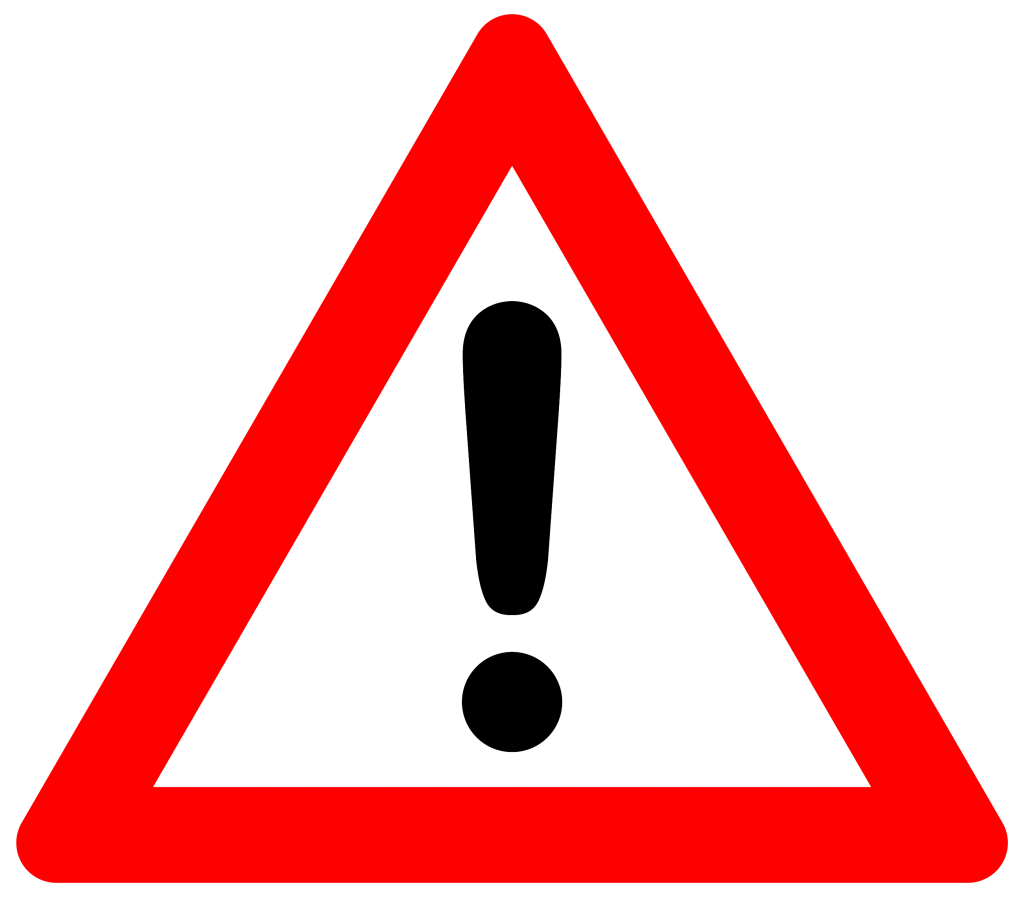
\includegraphics[scale=0.05]{Figures/triangle.png}
\end{figure}
\end{columns}
\end{frame}

\begin{frame}{Validità nei test italiani.}
\phantomsection\label{validituxe0-nei-test-italiani.}
\begin{columns}
\column{0.5\textwidth}

\vspace{2em}

\begin{figure}
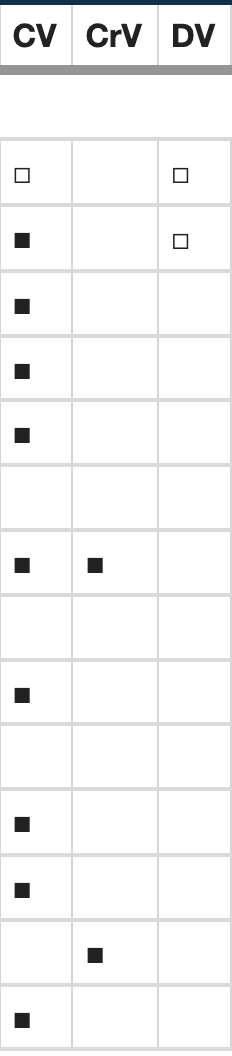
\includegraphics[scale=0.4]{Figures/Aiello_table.png}
\end{figure}

\column{0.5\textwidth}
Validità nei test di screening italiani (somministrazione dal vivo).
Aiello et al., 2022. Una cella senza quadratino indica che quel dato non è disponibile.

\vspace{2em}

CV=concurrent validity
CrV=criterion validity
DV=divergent validity

\end{columns}
\end{frame}

\begin{frame}{Un aspetto importante di validità}
\phantomsection\label{un-aspetto-importante-di-validituxe0}
\textbf{La validità non è qualità “immutabile” e data di un test}. ma
dipende da come lo si utilizza. Se il test viene utilizzato in maniera
inappropriata, allora può non diventare più valido.

L'appropriatezza dell'utilizzo di un test è determinata dall'adesione
alle procedure legate all'utilizzo del test stesso. Quanto più devio
dalle procedure iniziali e quanto meno valido è il test.

\pause

\textbf{NOTA:} queste considerazioni valgono per ogni strumento di
misurazione. Ci sono delle circostanze in cui può non funzionare bene.
Queste possono dipendere da ciò che misuriamo o dal nostro non
utilizzare in maniera adeguata le procedure che definiscono il test.
\end{frame}

\begin{frame}{Perdita di Validità 1/3}
\phantomsection\label{perdita-di-validituxe0-13}
Esempio da immagine del test ``Descrizione di Scene'' - APACS

\begin{center}
\includegraphics[width=0.6\linewidth,height=\textheight,keepaspectratio]{Figures/APACS_scene1.png}
\end{center}

è un test che misura l'efficacia comunicative, utilizzando come punto di
partenza la descrizione di una fotografia. Viene chiesto di dire dove si
è, chi c'è nella figura e cosa si sta facendo.
\end{frame}

\begin{frame}{Perdita di Validità 2/3}
\phantomsection\label{perdita-di-validituxe0-23}
Immaginate di stampare un'immagine con questa definizione. Oppure che
una persona abbia un problema di vista e veda questo.

\begin{center}
\includegraphics[width=0.6\linewidth,height=\textheight,keepaspectratio]{Figures/APACS_scene1.png}
\end{center}

Stiamo ancora misurando ciò che intendevamo?

Il test è ancora ``valido''?
\end{frame}

\begin{frame}{Perdita di Validità 1/3}
\phantomsection\label{perdita-di-validituxe0-13-1}
Questo esempio, un po' estremo, mostra come per una serie di ragioni, il
test potrebbe non misurare più quello che intendeva.

Idealmente dovremmo usare test che sono meno suscettibili a condizioni
in cui la validità è persa.

Il neuropsicologo forense dovrebbe essere attento a identificare se ci
sono situazioni che hanno fatto perdere validità al test. Di nuovo
questo sottolinea l'importanza dell' \emph{interpretazione} dei
punteggi.
\end{frame}

\begin{frame}{Esempio 1: MoCA e MMSE}
\phantomsection\label{esempio-1-moca-e-mmse}
\emph{Per che cosa è valido il MoCA?}

\hfill\break
Nell'identificare su cosa si basa un test, è comune fare l'errore di
bassarsi sull'intuito o solo sulla validità di facciata e non su altre
prove di validità.

\pause

Nel paper originale Nasreddine et al., 2005. Il MoCA era valido per
discriminare tra MCI, AD e, controlli.

Anche il MMSE (Folstein et al., 1975), nasceva per distinguere Demenze
da Depressione, ma è comunemente utilizzato come test generale di
funzionamento cognitivo.
\end{frame}

\begin{frame}{Esempio 2: Frontal Assessment Battery (FAB)}
\phantomsection\label{esempio-2-frontal-assessment-battery-fab}
\includegraphics[width=0.5\linewidth,height=\textheight,keepaspectratio]{Figures/FAB_validity.png}

Nell'articolo originale del 2005 (Appollonio et al.~2005) in realtà non
ci sono effettive prove di validità Questo non significa che il FAB-it
non abbia prove di validità per misurare funzioni esecutive(le versioni
di altre lingue del FAB le hanno), ma che di fatto non ci sono prove per
quella italiana.

(Prove della validità della FAB sono arrivate dopo, nel 2022, Aiello et
al., 2022), \textbf{sottolineando come la Validità sia un processo
continuo di accumulazione di evidenze.}
\end{frame}

\begin{frame}{Esempio 3:
{\small ABaCo Assessement BAttery for COmmunication} 1/2}
\phantomsection\label{esempio-3-12}
Il test ABACo per le valutazioni di capacità comunicative è un esempio
di eccellente test riguardo validità.
\end{frame}

\begin{frame}{Esempio 3:
{\small ABaCo Assessement BAttery for COmmunication} 2/2}
\phantomsection\label{esempio-3-22}
\begin{columns}
\column{0.5\textwidth}
\small
Validità del test ABaCo\\ (Sacco et al., 2008)

\column{0.5\textwidth}
\begin{figure}
\includegraphics[scale=0.3]{Figures/ABACO_validity.png}
\end{figure}
\end{columns}
\end{frame}

\section{Affidabilità}\label{affidabilituxe0}

\begin{frame}{Affidabilità}
\phantomsection\label{affidabilituxe0-1}
L'\textbf{Affidabilità} (o \textbf{Attendibilità}) è la qualità di un
test di fornire punteggi consistenti in diverse misurazioni, e può
essere quindi intesa come la precisione di un test.
\end{frame}

\begin{frame}{Tipi Affidabilità}
\phantomsection\label{tipi-affidabilituxe0}
\begin{itemize}
\tightlist
\item
  Affidabilità inter-rater
\item
  Affidabilità test-retest
\item
  Affidabilità Split-Half
\item
  Consistenza Interna
\end{itemize}

Esistono diverse classificazioni di affidabilità. Questa che sto
utilizzando è una delle possibili.
\end{frame}

\begin{frame}{Valori desiderabili}
\phantomsection\label{valori-desiderabili}
Spesso le misure di affidabilità sono associate a numeri. Le slide
seguenti ipotizzerò dei valori desiderabili di affidabilità che un test
dovrebbe avere.

È importante che questi sono valori ``indicativi'' e non esistono reali
valori considerati come standard nella letteratura. Per tale ragione
spesso circolano test con valori ben più bassi di quelli desiderabili.
\end{frame}

\begin{frame}{Affidabilità Inter-rater}
\phantomsection\label{affidabilituxe0-inter-rater}
\textbf{Affidabilità inter-rater}: è una misura della consistenza con
cui diversi esaminatori valutano la stessa prestazione dello stesso
paziente. É legata alla chiarezza istruzioni su come attribuire i
punteggi e alla complessità dei comportamenti osservati nel test.

Esistono vari modi di calcolarla. Nel metodo più diffuso è espressa da
un coefficiente, l'intraclass correlation, che varia tra 0 e 1, dove 0
indica completa inconsistenza tra i punteggi e 1 indica assoluta
consistenza tra i punteggi di due o più esaminatori.

Valori maggiori a 0.60 sono desiderabili.
\end{frame}

\begin{frame}{Affidabilità test-retest 1/4}
\phantomsection\label{affidabilituxe0-test-retest-14}
\textbf{Affidabilità test-retest}: rappresenta la correlazione di due
misure con lo stesso test effettuato dallo stesso esaminatore e sullo
stesso individuo dopo un intervallo di tempo \emph{in cui si assume che
non sia avvenuto nessun cambiamento.}

In genere è espressa da un coefficiente di correlazione che varia tra -1
e 1, Ma può essere anche espressa dal coefficiente ICC (lo stesso usato
per Inter-rater).

valori maggiori a 0.70 sono desiderabili
\end{frame}

\begin{frame}{Affidabilità test-retest 2/4}
\phantomsection\label{affidabilituxe0-test-retest-24}
Nota che l'affidabilità test-retest è sempre valutate con uno specifico
intervallo (es. 1 mese). Per tale ragioni esistono infinite possibili
affidabilità test-retest, dal momento che questo valore potrebbe variare
a seconda dell'intervallo.

Generalmente. Più corto è l'intervallo, più è probabile sia alta
l'affidabilità test-retest.
\end{frame}

\begin{frame}{Affidabilità test-retest 3/4}
\phantomsection\label{affidabilituxe0-test-retest-34}
\begin{columns}
\column{0.8\textwidth}
\small
\textbf{Se misurata con correlazione, l'affidabilità test-retest \textbf{non indica la stabilità del punteggio dei test nel tempo, o la possibilità di usarlo per fare valutazioni nel tempo.}} 

\column{0.2\textwidth}
\begin{figure}
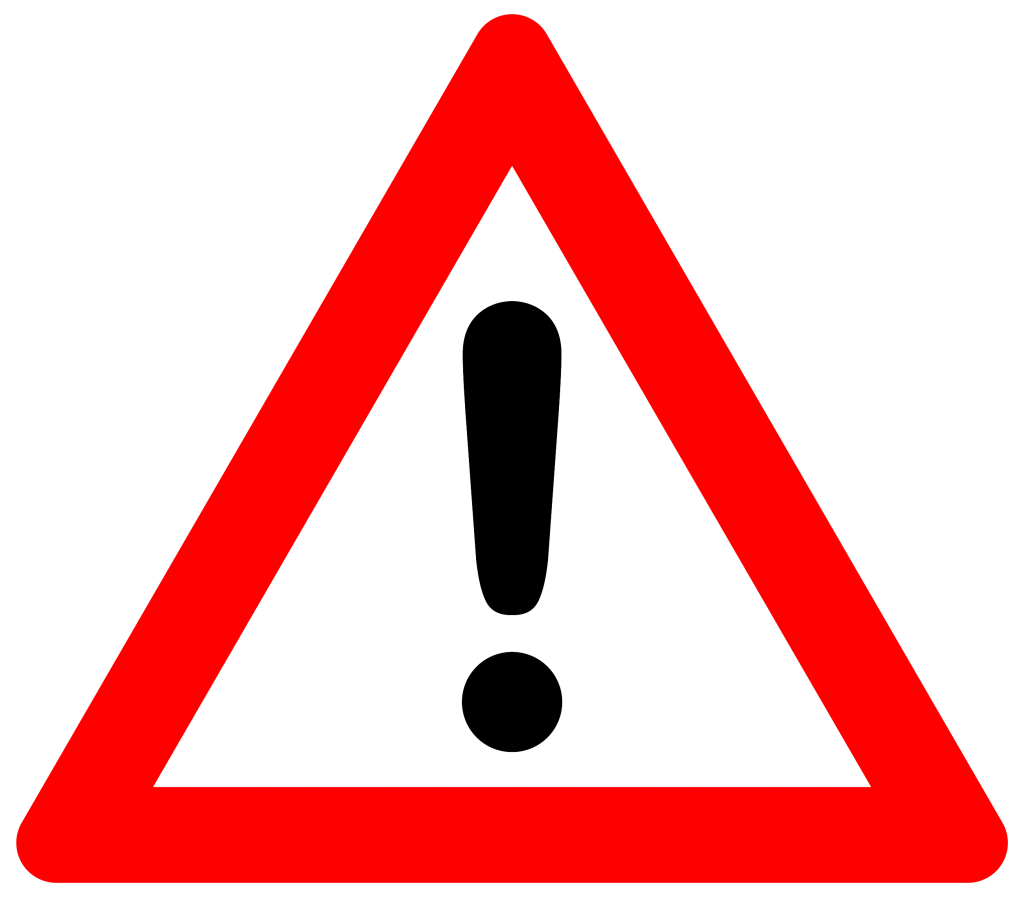
\includegraphics[scale=0.05]{Figures/triangle.png}
\end{figure}
\end{columns}
\end{frame}

\begin{frame}{Affidabilità test-retest 4/4}
\phantomsection\label{affidabilituxe0-test-retest-44}
Punteggi potrebbero avere una affidabilità test-retest (correlazione) di
0.98, ma essere poco stabili perché soggetti a \emph{variazioni
sistematiche}.

\pause

Più nello specifico. L'affidabilità test retest misurata tramite
correlazione non tiene conto dell'effetto pratica (trattata in slides
successive), visto che assume (anche matematicamente) che non ci siano
cambiamenti nel tempo. Questo aspetto sarà chiaro, studiando la formula
con cui è calcolato il test-retest, sia tramite simulazioni.
\end{frame}

\begin{frame}{Affidabilità Split-Half}
\phantomsection\label{affidabilituxe0-split-half}
L'affidabilità split-half stima l'affidabilità di un test misurando la
correlazioni tra due metà del test.

Il test viene diviso in due (metà degli item in una parte, metà
nell'altra) e viene calcolata una correlazione.

Valori maggiori a 0.70-0.80 sono desiderabili.
\end{frame}

\begin{frame}{Affidabilità Split-Half}
\phantomsection\label{affidabilituxe0-split-half-1}
L'affidabilità Split-half è meno dispendiosa da calcolare rispetto a
quella test-retest.

Il principale limite è che il risultato dipende molto dalla divisione
nelle metà (arbitraria.)
\end{frame}




\end{document}
